%%%%%%%%%%%%%%%%%%%%%%%%%%%%%%%%%%%%%%%%%%%%%%%%%%%%%%%%%%%%%%%%%
% Contents: Manta Input Device
% $Id: typeset.tex 537 2015-07-18 09:43:10Z oetiker $
%%%%%%%%%%%%%%%%%%%%%%%%%%%%%%%%%%%%%%%%%%%%%%%%%%%%%%%%%%%%%%%%%
\renewcommand{\chaptername}{Section}
\chapter{Manta Input Device}

\begin{intro}
  This section covers using a \emph{Manta} HOST device with particular
  focus on sequencer/composition mode.
\end{intro}

\section{Quickstart}

  Somehow condense everything to like 1-page of instruction to get up and going.


\section{Manta Presets}
  With a \emph{Manta} HOST device, the \emph{MantaMate's} 00-06 presets
  represent different ways the \emph{Manta} can be used as an instrument. The
  remaining 10-99 presets are user-saved.
   The active preset is shown on the \emph{MantaMate's} display.

  \begin{itemize}
    \item \texttt{00} Blank composition sequencer (default)
    \item \texttt{01} Monophonic controller
    \item \texttt{02} Duophonic controller
    \item \texttt{03} Triophonic controller
    \item \texttt{04} Tetraphonic controller
    \item \texttt{05} CV controller
    \item \texttt{06} Gate controller
    \item \texttt{07} Trigger controller
    \item \texttt{08-09} Unused
    \item \texttt{10-99} User-saved compositions.
  \end{itemize}

\section{Composition Preset}
  The 0 preset is the primary empty preset that can be used as a sequencer, keyboard, or
  direct trigger/gate/CV controller.

  When in a blank composition, the \emph{Manta} will default to a single sequencer
  that can have up to 32 steps activated. This mode will be referred to as
  Single-Sequence Pitched sequencer mode.

  \subsection{Getting Started/Basic Use}

  To get up and running with the \emph{Manta}, you will start in Play Mode. In play
  mode, you can press the lower hexes in order to add them to the sequence. All hexes
  added to the active sequence will be lit up amber.  Initially after pressing a hex,
  you can press the upper hexes and sliders to change that hexes
  values.

  \begin{figure}
    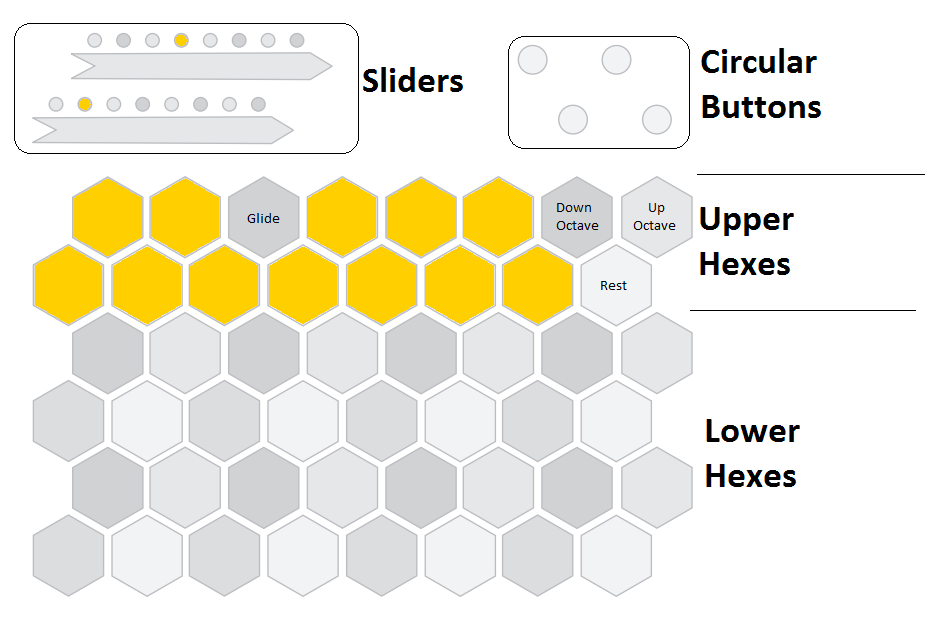
\includegraphics[width=\linewidth]{default.png}
  \end{figure}

  To further edit hexes that are already added, you can hit the top-right circular button
  and it will turn red to indicate you are in Edit Mode. You can now select hexes to edit
  their pitch and CV values, as well as the note length. If you would like to edit more
  than one hex value at once, you can multi-select in Edit Mode by holding a selected hex
  down and picking more hexes. Once you have selected a hex (or hexes, indicated by
  red LED), the list below covers all the values that can be changed for that
  hex (or hexes) and how to do so:
  \begin{itemize}
    \item 1V/O Pitch Class: Pick the note on the keybed presented
    on the upper hexes.
    \item 1V/O Octave: Press the top-right most hexes to transpose
    down or up and octave.

    \item CV1 Value: Press the top slider to change CV1 output value.
    \item CV2 Value: Press the bottom slider to change CV2 output value.
    \item CV3 Value: First, access the secondary CV values by pressing the top-left
    circular button until it is amber.
    Then, press the top slider to change CV3 output value.
    \item CV4 Value: First, access the secondary CV values by pressing the top-left
    circular button until it is amber.
    Then, press the bottom slider to change CV3 output value.

    \item Octave Value: First, access the access the misc. slider values by pressing
    the top-left circular button until it is red.
    Then, press the top slider to change to change the octave value.
    \item Note Length Value: First, access the access the misc. slider values by pressing
    the top-left circular button until it is red.
    Then, press the bottom slider to change to change the note length value.

    \item Pitch Glide Time: Press and hold the upper hex that lies between D\#
    and F\# to access the glide times. Press the upper slider to change the pitch
    glide time. Note this is the time to glide TO this note.
    \item CV Glide Time: Press and hold the upper hex that lies between D\#
    and F\# to access the glide times. Press the lower slider to change the CV
    glide time. Note this is the time to glide TO this hex CV value.
  \end{itemize}

  All the above values can be changed for each of the 32 hexes in the
  sequence. It should be noted that you actually have two sequencers running
  at once! Pressing the bottom-left circular button will turn it red and present
  you with the Menu Page. From here you can select Sequencer Mode and Order
  (covered below), but most importantly you can access the second sequencer by
  pressing the top-right most hex.

  The second sequencer (S2) acts similarly to the first (S1) but they run in parallel.

  Okay, so I've changed all these values, but now how do I get these values out of my
  \emph{MantaMate}?! First, we need to clock the \emph{MantaMate} from the ClkIn input
  (or use the internal clock, see: \ref{refInternalClock}).
  Then you can get the pitch/CV/gate from the respective outputs (where each cell
  represents a \emph{MantaMate} output):

  \begin{center}
  \begin{tabular}{ | m{1.5cm} | m{1.5cm}| m{1.5cm} | }
    \hline
    \texttt{S1: 1V/O} & \texttt{S1: Gate} & \texttt{S1: CV1} \\
    \hline
    \texttt{S1: CV2} & \texttt{S1: CV3} & \texttt{S1: CV4} \\
    \hline
    \texttt{S2: 1V/O} & \texttt{S2: Gate} & \texttt{S2: CV1} \\
    \hline
    \texttt{S2: CV2} & \texttt{S2: CV3} & \texttt{S2: CV4} \\
    \hline
  \end{tabular}
  \end{center}

  The gate out for each sequencer is the clock modified
  by the note length values of each hex, useful for triggering an ADSR or the like.


  \subsection{Left Option Menu}

  Fill in everything the left option menu does.

  Check out section 4 for possible copy-pasteable content from before the menu switch

  \subsection{Right Option Menu}

  Fill in everything the right option menu does

  \subsection{Sequencer Outputs}

  While using a \emph{Manta} host device, the \emph{MantaMate's} outputs are divided
  into to two separate sequencers. The first two rows of outputs are for the first
  sequencer, while the third and fourth rows are for sequencer two.

  The two sequencers can be changed to pitched, trigger, or even playable keyboard controller
  independently of each other.

  \subsubsection{Pitched Mode Outputs}

  Below outlines the \emph{MantaMate's} output of a sequencer when in pitched mode.
  Note, this output will correspond to row 1 and 2 if the first sequencer is in pitched
  mode, and 3 and 4 if the second sequencer is in pitched mode.


  \begin{center}
  \begin{tabular}{ | m{1.5cm} | m{1.5cm}| m{1.5cm} | }
    \hline
    \texttt{1V/O} & \texttt{Gate} & \texttt{CV1} \\
    \hline
    \texttt{CV2} & \texttt{CV3} & \texttt{CV4} \\
    \hline
  \end{tabular}
  \end{center}

  \subsubsection{Trigger Mode Outputs}
  Below outlines the \emph{MantaMate's} output of a sequencer when in trigger mode.
  Note, this output will correspond to row 1 and 2 if the first sequencer is in trigger
  mode, and 3 and 4 if the second sequencer is in trigger mode.

  \begin{center}
  \begin{tabular}{ | m{1.5cm} | m{1.5cm}| m{1.5cm} | }
    \hline
    \texttt{CV1} & \texttt{Trigger 1} & \texttt{Trigger 2} \\
    \hline
    \texttt{CV2} & \texttt{Trigger 3} & \texttt{Trigger 4} \\
    \hline
  \end{tabular}
  \end{center}


\subsection{Saving a Sequencer Pattern}

  Explain saving a sequencer pattern.

  WARNING: This only saves the sequence for your current session.
  If you would like to save a preset, see \ref{refSavingPreset}

\subsection{Saving a Preset} \label{refSavingPreset}

  Explain saving a preset.




\section{Preferences}

  In order to edit the preferences, hit the lower-right button labeled \texttt{P}.
  In order to access a subpreference, go to the corresponding preference menu
  and then hit the save button in the lower-right labeled \texttt{S}.

  While in any of the three preference menus, the lower-right LED will be lit.

  \subsection{Tuning and MIDI Learn}

  In order to enter this preference menu, hit the lower-right \texttt{P} once.

  \subsection{Glide}

  In order to enter this preference menu, hit the lower-right \texttt{P} twice.

  \subsection{Internal Clock}\label{refInternalClock}

  In order to enter this preference menu, hit the lower-right \texttt{P} three times.


\section{Monophonic Contoller Preset}

  Switching the \emph{MantaMate} to preset 01 sets it to the global
  Monophonic Controller Mode.

  The monophonic controller has an output for 1V/O, gate, as well
  as a CV that corresponds to the surface area coverage of the current
  hex.

  \begin{center}
  \begin{tabular}{ | m{1.5cm} | m{1.5cm}| m{1.5cm} | }
    \hline
    \texttt{V1: 1V/O} & \texttt{V1: Gate} & \texttt{V1: CV} \\
    \hline
    \texttt{Unused} & \texttt{Unused} & \texttt{Unused} \\
    \hline
    \texttt{Unused} & \texttt{Unused} & \texttt{Unused} \\
    \hline
    \texttt{Unused} & \texttt{Unused} & \texttt{Unused} \\
    \hline
  \end{tabular}
  \end{center}


\section{Duophonic Contoller Preset}

  Switching the \emph{MantaMate} to preset 02 sets it to the global
  Duophonic Controller Mode.

  The duophonic controller has two sets of outputs for 1V/O, gate, as well
  as a CV that corresponds to the surface area coverage of the current
  hex.

  \begin{center}
  \begin{tabular}{ | m{1.5cm} | m{1.5cm}| m{1.5cm} | }
    \hline
    \texttt{V1: 1V/O} & \texttt{V1: Gate} & \texttt{V1: CV} \\
    \hline
    \texttt{V2: 1V/O} & \texttt{V2: Gate} & \texttt{V2: CV} \\
    \hline
    \texttt{Unused} & \texttt{Unused} & \texttt{Unused} \\
    \hline
    \texttt{Unused} & \texttt{Unused} & \texttt{Unused} \\
    \hline
  \end{tabular}
  \end{center}


\section{Triophonic Contoller Preset}

  Switching the \emph{MantaMate} to preset 03 sets it to the global
  Triophonic Controller Mode.

  The triophonic controller has three sets of outputs for 1V/O, gate, as well
  as a CV that corresponds to the surface area coverage of the current
  hex.

  \begin{center}
  \begin{tabular}{ | m{1.5cm} | m{1.5cm}| m{1.5cm} | }
    \hline
    \texttt{V1: 1V/O} & \texttt{V1: Gate} & \texttt{V1: CV} \\
    \hline
    \texttt{V2: 1V/O} & \texttt{V2: Gate} & \texttt{V2: CV} \\
    \hline
    \texttt{V3: 1V/O} & \texttt{V3: Gate} & \texttt{V3: CV} \\
    \hline
    \texttt{Unused} & \texttt{Unused} & \texttt{Unused} \\
    \hline
  \end{tabular}
  \end{center}


\section{Tetraphonic Controller Preset}

  Switching the \emph{MantaMate} to preset 04 sets it to the global
  Tetraphonic Controller Mode.

  The tetraphonic controller has four sets of outputs for 1V/O, gate, as well
  as a CV that corresponds to the surface area coverage of the current
  hex.

  \begin{center}
  \begin{tabular}{ | m{1.5cm} | m{1.5cm}| m{1.5cm} | }
    \hline
    \texttt{V1: 1V/O} & \texttt{V1: Gate} & \texttt{V1: CV} \\
    \hline
    \texttt{V2: 1V/O} & \texttt{V2: Gate} & \texttt{V2: CV} \\
    \hline
    \texttt{V3: 1V/O} & \texttt{V3: Gate} & \texttt{V3: CV} \\
    \hline
    \texttt{V4: 1V/O} & \texttt{V4: Gate} & \texttt{V4: CV} \\
    \hline
  \end{tabular}
  \end{center}

\section{CV Contoller Preset}

  Switching the \emph{MantaMate} to preset 05 sets it to the global
  CV Controller Mode.

  The CV controller has twelve CV outputs corresponding to 12 hex surface
  area coverage.

  \begin{center}
  \begin{tabular}{ | m{1.5cm} | m{1.5cm}| m{1.5cm} | }
    \hline
    \texttt{CV} & \texttt{CV} & \texttt{CV} \\
    \hline
    \texttt{CV} & \texttt{CV} & \texttt{CV} \\
    \hline
    \texttt{CV} & \texttt{CV} & \texttt{CV} \\
    \hline
    \texttt{CV} & \texttt{CV} & \texttt{CV} \\
    \hline
  \end{tabular}
  \end{center}

\section{Gate Contoller Preset}

  Switching the \emph{MantaMate} to preset 06 sets it to the global
  Gate Controller Mode.

  The gate controller has twelve gate outputs corresponding to 12 hexes.

  \begin{center}
  \begin{tabular}{ | m{1.5cm} | m{1.5cm}| m{1.5cm} | }
    \hline
    \texttt{Gate} & \texttt{Gate} & \texttt{Gate} \\
    \hline
    \texttt{Gate} & \texttt{Gate} & \texttt{Gate} \\
    \hline
    \texttt{Gate} & \texttt{Gate} & \texttt{Gate} \\
    \hline
    \texttt{Gate} & \texttt{Gate} & \texttt{Gate} \\
    \hline
  \end{tabular}
  \end{center}

  \section{Trigger Contoller Preset}

    Switching the \emph{MantaMate} to preset 07 sets it to the global
    Trigger Controller Mode.

    The trigger controller has twelve trigger outputs corresponding to 12 hexes.

    \begin{center}
    \begin{tabular}{ | m{1.5cm} | m{1.5cm}| m{1.5cm} | }
      \hline
      \texttt{Trigger} & \texttt{Trigger} & \texttt{Trigger} \\
      \hline
      \texttt{Trigger} & \texttt{Trigger} & \texttt{Trigger} \\
      \hline
      \texttt{Trigger} & \texttt{Trigger} & \texttt{Trigger} \\
      \hline
      \texttt{Trigger} & \texttt{Trigger} & \texttt{Trigger} \\
      \hline
    \end{tabular}
    \end{center}

% Local Variables:
% TeX-master: "lshort2e"
% mode: latex
% mode: flyspell
% End:
